\usepackage{tikz}
\usepackage{pgfplots}
\pgfplotsset{compat=1.8}
\usetikzlibrary{arrows.meta,patterns,decorations.text,fit,calc}
\usepgfplotslibrary{statistics}

%\definecolor{smartgray}{gray}{0.55}
%\definecolor{smartred}{HTML}{800000}
%\definecolor{smartplum}{HTML}{47294F}
%\definecolor{smartblue}{HTML}{193A6B}
%\definecolor{smartorange}{HTML}{AA4C00}
%\definecolor{smartgreen}{HTML}{3C7705}
%\definecolor{smartbutter}{HTML}{A08300}

\definecolor{tangored}{HTML}{CC0000}
\definecolor{tangoplum}{HTML}{75507B}
\definecolor{tangoblue}{HTML}{3465A4}
\definecolor{tangoorange}{HTML}{F57900}
\definecolor{tangogreen}{HTML}{73D216}
\definecolor{tangobutter}{HTML}{EDD400}

\definecolor{aluminium1}{HTML}{EEEEEC}
\definecolor{aluminium2}{HTML}{D3D7CF}
\definecolor{aluminium3}{HTML}{BABDB6}
\definecolor{aluminium4}{HTML}{888A85}
\definecolor{aluminium5}{HTML}{555753}
\definecolor{aluminium6}{HTML}{2E3436}


\colorlet{class0c}{aluminium4}
\colorlet{class1c}{tangoplum}
\colorlet{class2c}{tangogreen}
\colorlet{class3c}{tangoorange}
\colorlet{class4c}{tangoblue}

\tikzstyle{classinv}=[draw=none, mark size=0pt]
\tikzstyle{class0}=[fill=class0c, draw=aluminium6,mark size=1pt]
\tikzstyle{class1}=[fill=class1c, draw=class1c!80!black,mark size=1pt]
\tikzstyle{class2}=[fill=class2c, draw=class2c!80!black,mark size=1pt]


\pgfmathdeclarefunction{invgauss}{2}{%
	\pgfmathparse{sqrt(-2*ln(#1))*cos(deg(2*pi*#2))}%
}

\pgfdeclarelayer{top}
\pgfsetlayers{main,top}

\newcommand{\labelsize}{\scriptsize}

\pgfplotsset{ticks=none,
	yticklabels=\empty,
	xticklabels=\empty,
	width=0.2\textwidth,
	height=0.2\textwidth,
	label style={font=\labelsize},
	%every label/.append style={text width=3em,align=center}
}

\newcommand{\plotdataOLD}[4]{
	\pgfmathsetseed{42}
	\addplot [#1,only marks, samples=10] ({invgauss(rnd,rnd)},{invgauss(rnd,rnd)});
	\addplot [#1,only marks, samples=5] ({1.5*invgauss(rnd,rnd)+#3},{invgauss(rnd,rnd)+\yshift});
	\addplot [#2, only marks, samples=10] ({invgauss(rnd,rnd)+#4},{invgauss(rnd,rnd)});
	\addplot [#2, only marks, samples=5] ({1.5*invgauss(rnd,rnd)+#3},{invgauss(rnd,rnd)+\yshift});
}

\newcommand{\plotdataset}[4][1]{
	\pgfmathsetseed{42}
	\addplot [#2,only marks, samples=10] ({invgauss(rnd,rnd)},{invgauss(rnd,rnd)});
	\addplot [#2,only marks, samples=5] ({1.5*invgauss(rnd,rnd)+#4},{invgauss(rnd,rnd)+#1*\yshift});
	\addplot [#3, only marks, samples=10] ({invgauss(rnd,rnd)+2*#4},{invgauss(rnd,rnd)});
	\addplot [#3, only marks, samples=5] ({1.5*invgauss(rnd,rnd)+#4},{invgauss(rnd,rnd)+#1*\yshift});
}

\newcommand{\plotProtos}{
	\addplot[only marks,class1,mark=diamond*,mark size=3pt](0,0);			
	\addplot[only marks,class2,mark=diamond*,mark size=3pt](2*\xshift,0);
	\draw[class1c] (axis cs:0,0) circle [radius=0.9*\xshift];
	\draw[class2c] (axis cs:2*\xshift,0) circle [radius=\xshift];
}

\newcommand{\plotOnlyProtos}{
	\addplot[only marks,class1,mark=diamond*,mark size=3pt](0,\protoshift);			
	\addplot[only marks,class2,mark=diamond*,mark size=3pt](2*\xshift,-\protoshift);
}

\newcommand{\plotSegment}[1][]{
	\pattern[pattern=north east lines, pattern color=class1c] (axis cs:-5,-5)--(axis cs:-5,0.5*\yshift)--(axis cs:\xshift,0.5*\yshift)--(axis cs:\xshift,-5)--cycle;
	\pattern[pattern=north west lines, pattern color=class2c] (axis cs:\xshift,-5)--(axis cs:\xshift,0.5*\yshift)--(axis cs:4*\xshift,0.5*\yshift)--(axis cs:4*\xshift,-5)--cycle;
	\ifthenelse{\equal{#1}{}}{}{
		%horizontal lines
		\pattern[pattern=vertical lines, pattern color=class0c] (axis cs:-5,0.5*\yshift)--(axis cs:-5,2*\yshift)--(axis cs:4*\xshift,2*\yshift)--(axis cs:4*\xshift,0.5*\yshift)--cycle;
	}
}


\def\xshift{3.5}
\def\yshift{8}
\def\protoshift{0.5}

\newcommand{\tikzvoodoo}{
	\begin{tikzpicture}[
		node distance=3em,
		%	minimum size =0.15\textwidth,
		%	very thick,
		from/.style={{Stealth[length=0.8em, round]}-,double,shorten >=-0.2em,shorten <=-0.2em},
		towards/.style={-{Stealth[length=0.8em, round]},double,shorten >=-0.2em,shorten <=-0.2em},
		]
		%		\node(img1a) at (0,0) {};
		%		\node[label=below:Befor Drift](img1a) {%
			\node(beforedrift) {%
				\begin{tikzpicture}
					\begin{axis}[xlabel={before drift}]
						\plotdataset{class1}{classinv}{\xshift}
					\end{axis}
				\end{tikzpicture}
			};
			%		\node[label=below:After Drift] (img1b) [below=of img1a] {%
				\node(afterdrift) [node distance=0em, below=of beforedrift] {%	
					\begin{tikzpicture}
						\begin{axis}[xlabel={after drift}]
							\plotdataset{classinv}{class2}{\xshift}
						\end{axis}
					\end{tikzpicture}
				};
				\draw[decorate,decoration={brace,amplitude=1.5em,mirror,raise=-0.3em}] (beforedrift.north west) -- node[xshift=-1.2em](leftdrift){} (afterdrift.south west);
				\draw[decorate,decoration={brace,amplitude=1.5em,raise=-0.3em}] (beforedrift.north east) -- node[xshift=1.2em](rightdrift){} (afterdrift.south east);	
				%	\node[label=below:stream](stream) [below left=of leftdrift] {%
					\node(stream) [below left=of leftdrift] {%
						\begin{tikzpicture}
							\begin{axis}[xlabel={}]
								\plotdataset{class0}{class0}{\xshift}
							\end{axis}
						\end{tikzpicture}
					} edge[towards]
					[postaction={decoration={text along path, text align=center,text={|\labelsize |drift ||},
							raise=0.2em,},decorate}]
					[postaction={decoration={text along path, text align=center,text={|\labelsize |detection ||},
							raise=-0.7em,}, decorate}]
					(leftdrift);
					\node[node distance=0em,below=of stream] {stream};
					%%
					%%  drifting Area
					%%
					\node(driftingarea) [right=of rightdrift] {
						\begin{tikzpicture}
							\begin{axis}
								\plotdataset{class1}{class2}{\xshift}
								\plotSegment
							\end{axis}
						\end{tikzpicture}
					} edge [from] node[above]{\labelsize train} 
					node[below]{\labelsize model} (rightdrift);
					\node[node distance=0em,below=of driftingarea,font=\labelsize,align=center] {drift \\[-0.5em] locus};
					%%
					%%  Global Explanation
					%%
					\node (nopreproc) [right=of driftingarea] {
						\begin{tikzpicture}
							%[hide y axis,axis x line*=bottom]
							\begin{axis}[axis line style={white,}]
								\plotdataset{classinv}{classinv}{\xshift}
							\end{axis}
						\end{tikzpicture}
					} edge [from] (driftingarea);
				    \node at (nopreproc) {\Huge $\bullet$};
					%%
					%%  DiDi
					%%
					\node[label=east:DiDi] (didi) [right=of nopreproc] {
						\begin{tikzpicture}
							\begin{axis}
								\plotdataset[2]{class1}{class2}{4*\xshift}
							\end{axis}
						\end{tikzpicture}
					} edge [from] (nopreproc);
					%%
					%%  WBM
					%%
					\node[label=east:WBM] (wbm) [node distance=0em, above=of didi] {
						\resizebox{.1\textwidth}{!}{
							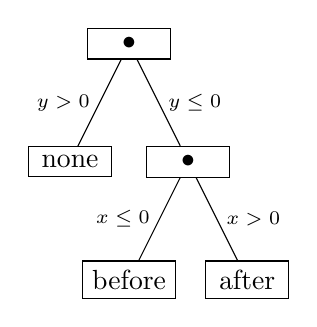
\begin{tikzpicture}
								\begin{scope}[X/.style={draw,minimum width=3em}]
									\node[X] {$\bullet$}
									child {node[X] {none} edge from parent node[left] {\labelsize $y>0$}}
									child {node[X] {$\bullet$}
										child {node[X] {before} edge from parent node[left] {\labelsize $x\leq0$}}
										child {node[X] {after}edge from parent node[right] {\labelsize $x>0$}}
										edge from parent node[right] {\labelsize $y\leq0$}};
								\end{scope}
							\end{tikzpicture}
						}
					} edge [from] (nopreproc);
					%%
					%%  PFI
					%%
					\node[label=east:PFI] (pfi) [node distance=0em,below=of didi] {
						%	\resizebox{.1\textwidth}{!}{
							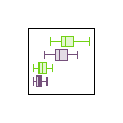
\begin{tikzpicture}
								\begin{axis}[
									boxplot/draw direction=x,
									ymin=0,ymax=5,%ymajorticks=true,
									cycle list={{class1c},{class2c}},
									tick align=inside,
									ytick={1,2,3,4},
									yticklabels={$z_2$,$z_1$,$y$,$x$},
									]
									%box for z2
									\addplot+[fill,fill opacity=0.2,
									boxplot prepared={
										median=2,
										upper quartile=2.35,
										lower quartile=1.5,
										upper whisker=3.4,
										lower whisker=1.1
									},
									] coordinates {};
									%box for z1
									\addplot+[fill,fill opacity=0.2,
									boxplot prepared={
										median=2.59,
										upper quartile=3.35,
										lower quartile=2,
										upper whisker=4.4,
										lower whisker=1.1
									},
									] coordinates {};
									%box for y
									\addplot+[fill,fill opacity=0.2,
									boxplot prepared={
										median=5.57,
										upper quartile=6.93,
										lower quartile=4.93,
										upper whisker=8.68,
										lower whisker=3.03
									},
									] coordinates {};
									%box for x
									\addplot+[fill,fill opacity=0.2,
									boxplot prepared={
										median=6.57,
										upper quartile=7.93,
										lower quartile=5.93,
										upper whisker=10.68,
										lower whisker=4.03
									},
									] coordinates {};
									%		\addplot+[xbar] coordinates {
										%				(1,1) 
										%				(2,2) 
										%				(3,3) 
										%				(0,4)
										%			};
								\end{axis}
							\end{tikzpicture}
							%}
					} edge [from] (nopreproc);
					%%
					%%  CFs
					%%
					\node[label=east:CF] (cf) [node distance=0em,below=of pfi] {
						\begin{tikzpicture}
							\begin{axis}
								\plotdataset{class1}{class2}{\xshift}
								\plotSegment
								\plotOnlyProtos
								%\plotProtos
								\begin{pgfonlayer}{top}
									\draw[class1c!80!black,-{Stealth}] (axis cs:0,\protoshift) to [bend left] (axis cs:1.1*\xshift,\protoshift) node[above,midway,black] {};
									\draw[class2c!80!black,-{Stealth}] (axis cs:2*\xshift,-\protoshift) to [bend left] (axis cs:0.8*\xshift,-\protoshift) node[above,midway,black] {};
									\addplot[only marks,class1,mark=triangle*,mark size=2.5pt](1.1*\xshift,\protoshift);			
									\addplot[only marks,class2,mark=triangle*,mark size=2.5pt](0.8*\xshift,-\protoshift);
								\end{pgfonlayer}
							\end{axis}
						\end{tikzpicture}
					};
					%%
					%%  LIME
					%%
					\node[label=east:LIME] (lime) [node distance=0em, below=of cf] {
						\begin{tikzpicture}
							\begin{axis}
								\plotdataset{class1}{class2}{\xshift}
								\plotSegment
								\plotOnlyProtos
								%\plotProtos
								\begin{pgfonlayer}{top}
									\draw[class1c!80!black,-{Stealth}] (axis cs:0,\protoshift) -- (axis cs:0.8*\xshift,\protoshift) node[above,near start,black] {\tiny $\partial_1$}; %,yshift=-0.3em
									\draw[class2c!80!black,-{Stealth}] (axis cs:2*\xshift,-\protoshift) -- (axis cs:1.2*\xshift,-\protoshift) node[above,near start,black] {\tiny $\partial_2$}; %midway,yshift=-0.3em
								\end{pgfonlayer}
							\end{axis}
						\end{tikzpicture}
					};% edge [from] (img3b);
					%%
					%%  Rep Prototypes
					%% ($(x1.east)!0.5!(xm.west) + (0,1.5cm)$) 
					\node[node distance=0em] (mid) at ($(cf.west)!0.5!(lime.west)$) {};
					%	\node (repproto) [left =of cf] {	
						\node (repproto) at (nopreproc |- mid) {
							\begin{tikzpicture}
								\begin{axis}
									\plotdataset{class1}{class2}{\xshift}
									\plotSegment
									\plotOnlyProtos
									%\plotProtos
								\end{axis}
							\end{tikzpicture}
						} edge [from] (driftingarea);
						\node[node distance=0em,below=of repproto,font=\labelsize,align=center] {representing \\[-0.5em] prototypes};
						\draw (repproto) edge[towards] (cf);
						\draw (repproto) edge[towards] (lime);
						\node (segmentation) [left =of repproto] {
							\begin{tikzpicture}
								\begin{axis}
									\plotdataset{class1}{class2}{\xshift}
									\plotSegment[1]
								\end{axis}
							\end{tikzpicture}
						} edge [towards] (nopreproc);
						\node[node distance=0em,below=of segmentation,font=\labelsize,align=center] {drift \\[-0.5em] segmentation};
						\draw (segmentation) edge [towards] (repproto);
						\node[below right=of stream] {};·
%						\node (betweenDriftLow) at ($(driftingarea) !0.5! (nopreproc)$){B};
						\node (betweenPfiCf) at ($(pfi.east) !0.5! (cf.east)$) {};
						\node (betweenPfiCfShifted) at ($(betweenPfiCf) + (-20em,0)$) {};
						\draw(stream) edge [towards,out=315,in=180] (segmentation);
						\node[fit=(leftdrift) (beforedrift) (betweenPfiCfShifted) (driftingarea),inner ysep=0em,inner xsep=0.85em] (loc) {}; %
						\node[fit=(segmentation) (loc.south west) (loc.south east),inner ysep=1.7em,inner xsep=0em] (seg) {};
						\draw[dashed,class0c] (loc.north west) -- (seg.south west);
						\draw[dashed,class0c] (loc.south west) -- (betweenPfiCf);%(loc.south east);
						\draw[dashed,class0c] (loc.north east) -- (seg.south east);
						\node[node distance=-0.5em,below=of loc,anchor=south west] (textLoc) {localization};
						\node[node distance=0.5em,below=of loc,anchor=north west] (textSeg) {segmentation};
						\node[anchor=west] at ($(nopreproc.west |- textLoc) + (0.5em,0)$) {global}; %[align=left]
						\node[anchor=west] at ($(nopreproc.west |- textSeg) + (0.5em,0)$) {local};
						
						%	\node[below=of sum, anchor=west,align=right,text width=3.5em] (eps1) {$\privloss_1$};
						%	\node[anchor=west,align=right,text width=3em] at ($(eps1 -| gradient)$) (eps2) {$\privloss_2$};	
					\end{tikzpicture}
				}
